\documentclass[a4j,10pt,twocolumn]{../styles/utf8/abstract}
%\documentclass[a4j,9pt,twocolumn]{abstract}

\usepackage[dvipdfmx]{graphicx}
\usepackage{latexsym}
\usepackage{amssymb}
\usepackage{float}
\usepackage{enumerate,cite,url}
\usepackage{color}
\usepackage{listings,jlisting}
\lstset{%
    language={c},%
    basicstyle={\small\ttfamily},%
    identifierstyle={\small},%
    commentstyle={\footnotesize\itshape},%
    keywordstyle={\small},%\bfseries},%
    ndkeywordstyle={\small},%
    stringstyle={\small\it},
    frame={tb},
    breaklines=true,
    columns=[l]{fullflexible},%
    numbers=left,%
    xrightmargin=0zw,%
    xleftmargin=3zw,%
    numberstyle={\scriptsize},%
    stepnumber=1,
    numbersep=1zw,%
    lineskip=-0.5ex%
}

\title{Component-Based Software Development Framework\\for Embedded IoT Devices}	% 論文のタイトル
\author{山本 拓朗} 		% 著者
\studentid{29C16100} 	% 学籍番号
\lab{潮}		% 研究室名

% 英語なら以下2行を定義
\englishtitle
\jptitle{{\Large 組込みIoTデバイス向けコンポーネントベースソフトウェア開発フレームワーク}}  % 日本語のタイトル

\begin{document}
\absttitle 		% 表題の出力

\section{緒論}

近年,IoT (Internet of Things) 市場の拡大により,組込み機器をネットワークに繋げて操作するために,ソフトウェア開発の高い生産性が要求されている.
組込みソフトウェア開発の生産性向上のため,スクリプト言語mruby (軽量Ruby) を用いたコンポーネントベース開発が可能なフレームワークmruby on TECS\cite{par:mrubyonTECS}が提案されている.

本研究では,IoT機器に対応するため,mruby on TECS の拡張として組込み向けTCP/IPプロトコルスタックTINET の機能をmrubyプログラムから実行できるフレームワークを提案する.
提案フレームワークでは,TINETのコンポーネント化を行うことで拡張性やコンフィグラビリティが向上し,プロトコルを容易に設定できるようになる.
さらに,動的メモリアロケータTLSF (Two-Level Segregate Fit) のコンポーネント化も行い,スレッドセーフに複数のスレッドを動作可能なメモリアロケータもフレームワークに組み込んでいる.

\section{mruby on TECS}

mruby on TECS は,スクリプト言語mrubyと,組込みシステムに適したコンポーネントシステムであるTECS (TOPPERS Embedded Component System) を組み合わせたフレームワークである.
スクリプト言語はその使いやすさから生産性が高い反面,C 言語に比べると実行速度が遅いため,組込みシステムに適用することは難しい.
mruby on TECS では,mrubyブリッジというmrubyプログラムからC 言語の関数を呼び出す機能を提供しており,mrubyに比べて,アプリケーションを約100 倍速く実行できる.

さらに,TECSによってコンポーネントベースで開発されているため,ソフトウェアの再利用が高く,機能の追加や取り外しが容易である.

\section{提案フレームワーク}

提案フレームワークでは,mruby on TECSを拡張して,TCP/IPプロトコルスタックTINET+TECSと動的メモリアロケータTLSF+TECSの設計・実装を行った.
図\ref{fig:SystemModel}に提案フレームワークのシステムモデルを示す.

TINET+TECSは,TECSによりTINETをコンポーネント化した組込みシステム向けTCP/IPプロトコルスタックである.
TINETは組込みシステムに適したコンパクトなTCP/IPプロトコルであるが,多くの複雑なソースコードやマクロのせいでコンフィグラビリティが低く,メンテナンスや拡張・検証が難しい.
TINET+TECSでは,プロトコルの各層をコンポーネントとして実装しているため,TCP層やUDP層の付け外し,IPv4とIPv6の共存,通信用バッファのサイズ変更など,プロトコルの設定が既存のTINETに比べて容易になっている.

\begin{figure}[h]
    \centering
    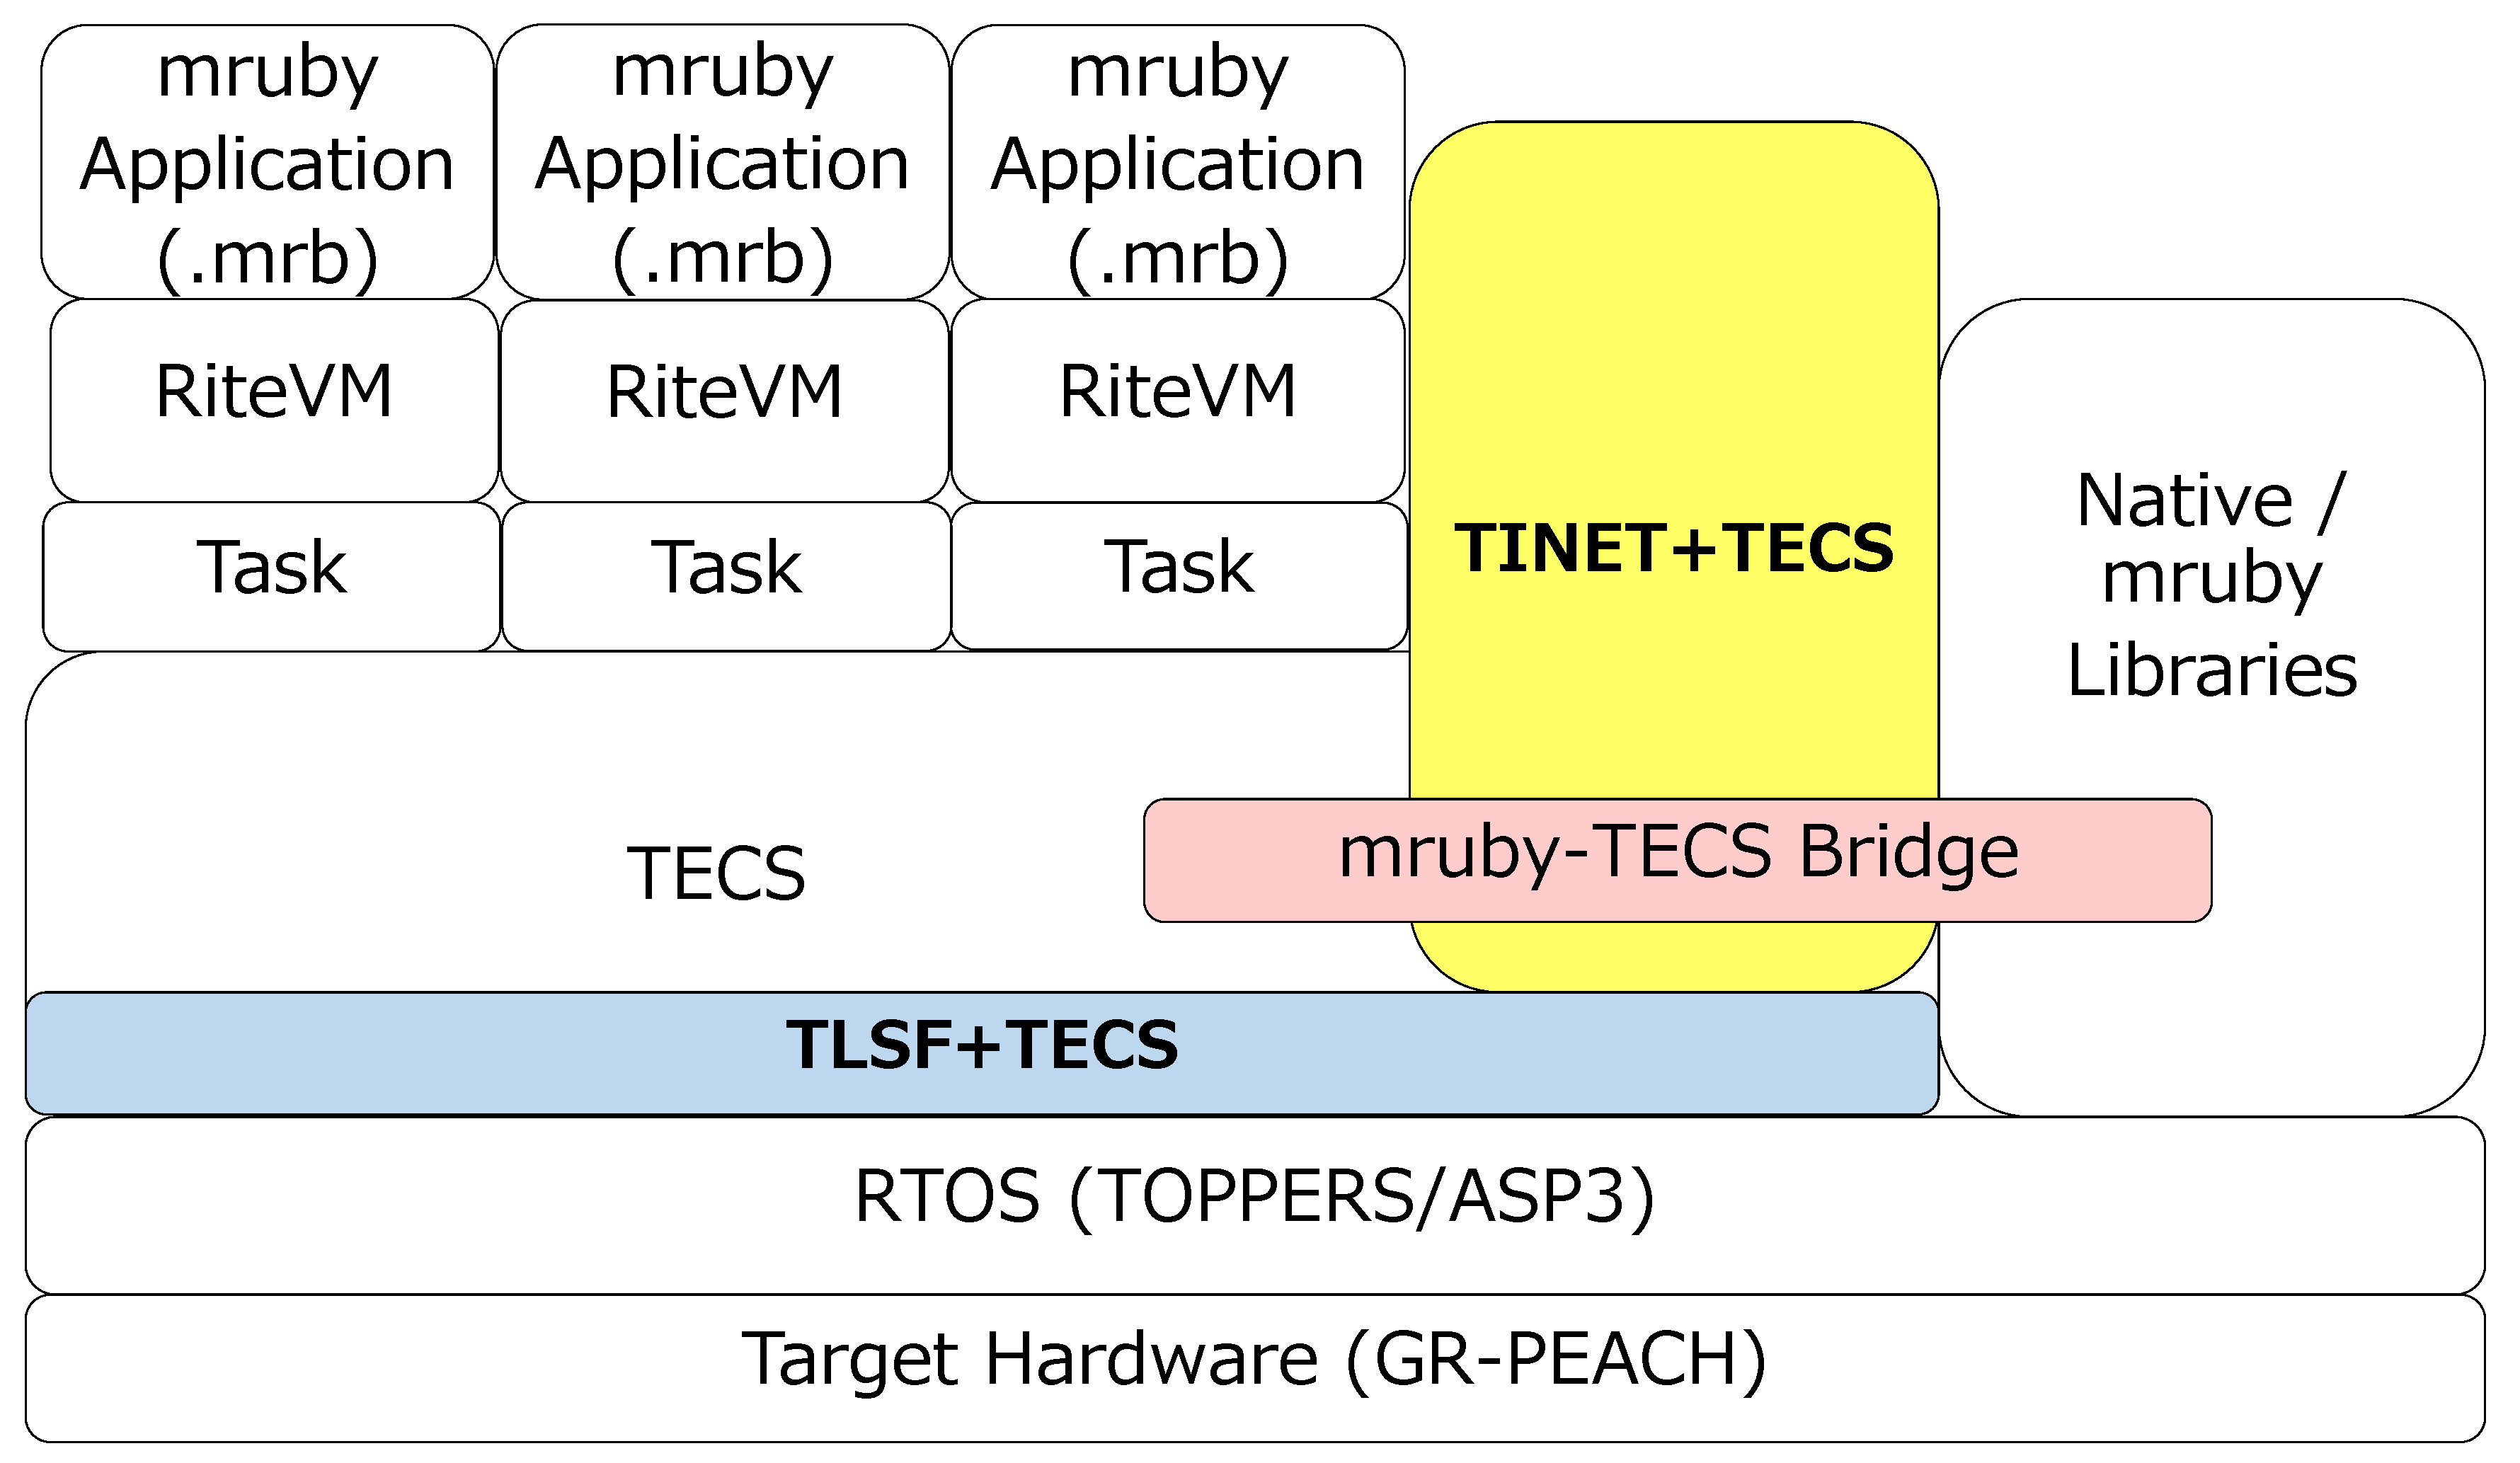
\includegraphics[width=8cm,clip]{SystemModel.pdf}
    \vspace{-0.2cm}
    \caption{システムモデル}
    \vspace{-0.4cm}
    \label{fig:SystemModel}
\end{figure}

TLSF+TECSは,TECSによりTLSFをコンポーネント化した組込みシステム向け動的メモリアロケータである.
TLSFはメモリ利用効率が良く常に$O(1)$で動作する高速なアロケータであるが,複数のスレッドが並行動作すると,メモリ競合が起きる場合がある.
TLSF+TECSでは,TLSFコンポーネントが独自のヒープ領域を保持するため,排他制御なしで複数のスレッドを動作させることができる.
さらに,コンポーネントの特性により,ヒープメモリのサイズ変更が柔軟になる.

図\ref{src:Application}は,提案フレームワーク上で動作させるアプリケーションの例(1秒周期でセンサデータを取得し,サーバへ送信する)を示している.
mrubyプログラムからTINETの機能を利用でき,IoTデバイスに適用できるネットワークソフトウェアを開発できる.

\begin{figure}[t]
\centering
\begin{lstlisting}
begin
    io = AnalogIO.new(A0, INPUT)
    cep = TCP.new()
    cep.accept
    loop do
        val = io.read
        cep.snd val.to_s + "\n"
        RTOS.delay(1000)
    end
rescue => e
    puts "[ERROR]" + e
end
\end{lstlisting}
\vspace{-0.2cm}
\caption{提案フレームワークでのアプリケーション例}  
\vspace{-0.7cm}
\label{src:Application}
\end{figure}

\section{結論}

mruby on TECS フレームワークの拡張として,IoTデバイス向けのソフトウェアを開発するフレームワークを提案した.
提案フレームワークでは,TCP/IPプロトコルスタックであるTINETの機能をmrubyプログラムから呼び出せる.
さらに,ソフトウェアコンポーネントとしてTINET+TECSとTLSF+TECSを実装し,コンポーネント化によるソフトウェア開発の生産性向上を示した.

%\bibliographystyle{junsrt}
%\bibliography{refs}
\begin{thebibliography}{1}
\bibitem{par:mrubyonTECS}
    T. Azumi, Y. Nagahara, H. Oyama, and N. Nishio, 
    ``mruby on TECS: Component-Based Framework for Running Script Program," 
    in Proc. of IEEE ISORC, 
    pp.252-259, 
    2015. 
\end{thebibliography}
\newpage
\pagebreak
\end{document}
